\documentclass[11pt]{article}

\usepackage{fullpage}
\usepackage[usenames,dvipsnames]{xcolor}
\usepackage{amsmath}
\usepackage{graphicx}
\usepackage{wrapfig}


\begin{document}
\begin{center}

\color{RoyalPurple} \textbf{\Large Statistics ... Lurking Around Every Corner}

\end{center}

\color{black}

Statistics is a very useful field though frequently disliked, even at times by those in the mathematical community. Statistics brings with it a great need for ethics and transparency. I was once told by a teacher “\textit{statistics in the hands of a stupid man is dangerous}”. However, statistics is used regularly in many fields. It has become a necessary part of computer sciences even branching off into its own sub-field of data sciences. The entire field of data science would not exist without statistics. In your everyday life, statistics and probability are at work in many avenues you may not even realize. Every time you drive your car there is a probability of being in an accident. When you get home you face the likelihood that someone may have burglarized your home. It is simply inescapable, probability and statistics is in action everywhere around you. 

\bigskip

\bigskip

\noindent \color{RoyalPurple} \textbf{\large Probability in Home Entertainment}

\bigskip

\color{black}

A favorite past time of many is playing card games. No matter what card game you play, you're playing with probability. Of all the statistics formulas probability is usually the easiest to understand.
\color{OliveGreen}
$$ \text{Probability} = \frac{\text{events}}{\text{outcomes}} $$ 

\color{black}
\bigskip
\noindent Each card laid in “the river” in Texas Hold’em (a popular variation of Poker) has a probability of appearing depending on the cards already dealt. Each possible combination forming a winning hand (flush, straight, 3 of a kind, etc.), has an associated probability based on what has already been laid, and what is in the other players hands.$^1$ Probability can quickly get more complex. However, if you understand the basic idea, more complicated probabilities are quickly mastered. 

\bigskip

To demonstrate, imagine that you have a hand containing an Ace of Spades and an Ace of Hearts, the rest of the deck of cards (minus the two Jokers) sits in front of you. What is the probability that you will draw another Ace from the deck on the next draw? There are 52 cards in a deck (excluding the Jokers), and there are 4 aces (clubs, spades, hearts, diamonds). That means that there are 2 aces left in the deck which now contains 50 cards. Therefore, the chance (or probability) of picking another ace from the deck is: 

\bigskip
\color{OliveGreen}
$$ \text{Probability} = \frac{\text{remaining aces}}{\text{remaining cards}} = \frac{2}{50} = \frac{1}{25} = 0.04 $$
\color{black}
\bigskip

All home games (video games included) are very heavily reliant on the probability of a specific outcome, even if it is only the roll of a die. Even in word games such as scrabble you have the probability of picking a certain letter out of the bag. The chance you take in each draw is part of the fun.

\newpage

\noindent \color{RoyalPurple} \textbf{\large Statistics in Services}

\color{black}
\bigskip

Starting again with probability let's examine how many ways probability is affecting your life when you may not even be aware of it. For example, your insurance premiums (be it car, home, or life) are calculated using detailed models called risk models to determine the cost to you. This includes several variables which are used to calculate the likelihood of a payout by the insurance company. Let's look at a simple example of a model to give you a better idea of the concept. The following is called the collective risk model.$^2$ This model uses the Greek letter capital sigma ($\sum$) which is used to denote a summation which is the continued adding of N items starting from the index i. This summation is then used in an even larger, more complex model used to compute the likelihood of a payout, and eventually the premium at which you should be charged in order to cover the cost of any likely payout. \color{OliveGreen}

$$ S_t = \sum_{i=1}^{N_t}X_{t,i} $$

\noindent Where $S_t$ is the large number of aggregate claims,  \textit{t} indicates time, N$_t$ is the frequency of claims of a specific account in the period \textit{t} time, $X_{t,i}$ is the $i^{th}$ amount amount of a claim which occurred in the period \textit{t} time.

\bigskip	
\color{black}	
There is an entire field built around models such as this, called the Actuarial Sciences which is the study and evaluation of risk. People who specialize in such sciences are consultants, analysts and work in insurance, finance, or consulting firms. You've probably heard of a risk analyst that would calculate a specific risk in order to mitigate possible losses. 

\bigskip

\bigskip

\noindent \color{RoyalPurple} \textbf{\large Statistics in Everyday Life}

\bigskip
\color{black}

What has a greater impact on your everyday life than the weather. The chance of snow or flooding can impact school and work closure. Even on a more basic level, if you know there is a high percent for a chance of rain, you are more likely to bring an umbrella, wear a raincoat, or maybe opt for waterproof footwear instead of flip flops. Weather forecasting is very dependent on statistical analysis. In fact, weather is even more closely related to the data sciences, or applied statistics. Nowadays weather data has been gathered for decades. The data is compiled and used to predict future weather patterns.$^3$ 

\bigskip
Weather forecasting frequently uses numerous statistical methods. For simplicity we will look at the basic models behind the types of models that are typically used. This is because some of the models used for weather forecasting requires the understanding of complicated weather terminology are more advanced mathematical terms than it would be efficient to explain in this paper. The most popular statistical methods used in forecasting are simple and multiple linear regressions. A simple linear regression looks at the relationship between independent and dependent variables using a straight line (or line of best fit) to determine the correlation. The slope of the line will be negative or positive showing the type of correlation between the variables. In other words, a positive slope indicates that as the independent variable increases, the average (or mean value) of the dependent variable also increases. The regression line pictured below$^4$ can be seen to have a positive slope, therefore showing a positive correlation between variables. A multiple linear regression is very similar, the only difference being two or more independent variables. This could be used to measure multiple continuous variables such as humidity, rainfall, and temperature with the same continuous dependent variable. In the figure below, notice the solid black line, this would be the line of best fit or the regression line.
\bigskip
 
\begin{center}
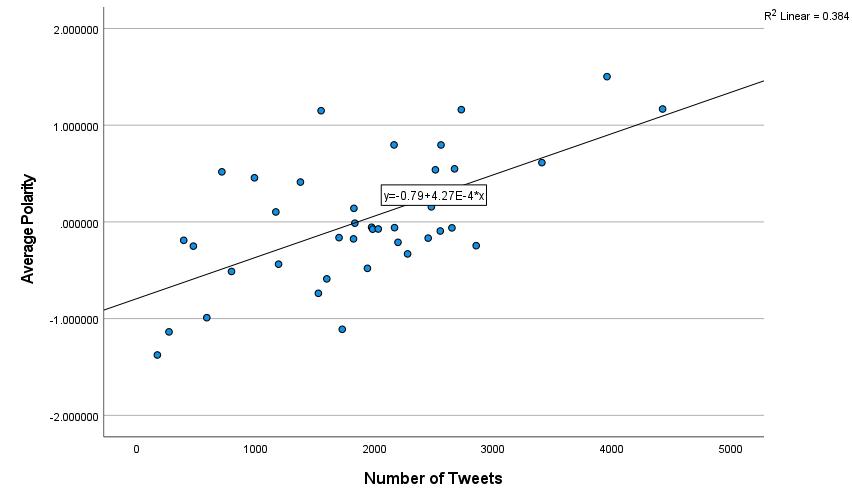
\includegraphics[scale=.75]{ScatterPlot}
\end{center}

\bigskip

Clearly statistics exists in many aspect of our everyday lives. It truly does lurk behind every corner. Looking on the bright side, statistics and probability is there whether you choose to notice it or not. Though, having even a basic understanding of statistics can help to improve your chance of winning family game night. It can also prepare you for possible premium hikes in your insurance due to making a claim. Most importantly it can help to avoid ruining your brand new suede booties by being prepared to be out in the rain. 

\vspace{1in}
\begin{center}
Bernadette Hoffman \\
Math 408\\
03/15/22\\
Created using \LaTeX.
\end{center}

\newpage
\begin{center}
\Large \textbf{References}
\end{center}

\bigskip

\begin{small}

\noindent $^1$“Texas Holdem Poker: Poker Rules.” \textit{PokerNews}, 
https://www.pokernews.com/poker-rules/texas-holdem.htm.

\bigskip

\noindent $^2$Lesmana, E., et al. "Model estimation of claim risk and premium for motor vehicle insurance by using Bayesian method." \textit{IOP Conference Series: Materials Science and Engineering}. Vol. 300. No. 1. IOP Publishing, 2018. doi:10.1088/1757-899X/300/1/012027

\bigskip

\noindent $^3$Agbo, Emmanuel P. “The Role of Statistical Methods and Tools for Weather Forecasting and Modeling.” \textit{Weather Forecasting}, 28 Oct. 2020, https://doi.org/10.5772/intechopen.96854.

\bigskip

\noindent $^4$Meteorological Development Lab, “Probability Distribution Forecasts of a Continuous Variable”, National Weather Service, Oct. 2007, https://www.weather.gov/media/mdl/Peroutka_Oct03_2007.pdf

\bigskip

\noindent “Beyond Barometers: How Statistics Helps Predict the Weather.” \textit{This Is Statistics}, 25 Jan. 2018, \\
https://thisisstatistics.org/beyond-barometers-how-statisticians-help-to-predict-the-weather/.

\end{small}

\end{document}